\chapter*{前言与阅读路线图}
\markboth{\sffamily\slshape Preface}
{\sffamily\slshape Preface}


扩散模型已迅速成为生成式建模的核心范式，其大量研究工作横跨机器学习、计算机视觉、自然语言处理等众多领域。这些文献散布于不同社区，并凸显了进展的多个维度，包括：涉及建模原理、训练目标、采样器设计及其背后数学思想的理论基础；涵盖工程实践和架构选择的实现进展；将模型适配到特定领域或任务的实际应用；以及在计算、内存和部署效率上进行改进的系统级优化。


本书旨在为扩散模型提供一个\emph{有原理的基础}，聚焦于以下核心主题：
\begin{itemize}
    \item 我们呈现支撑扩散模型研究的核心概念和公式，为读者提供理解更广泛文献所需的核心知识。我们并不综述所有变体或领域特定的应用，而是建立稳定的概念基础，由此可以理解各类后续发展。
    \item 与从噪声到数据学习直接映射的经典生成式模型不同，扩散模型将生成视为随时间渐进的变换，将粗略结构逐步精炼为精细细节。这一核心思想通过三种主要视角发展而来，即\emph{变分}、\emph{分数}和\emph{流}方法，它们为理解和实现扩散建模提供了互补的途径。我们聚焦于这些公式的核心原理与基础，旨在追溯其关键思想的起源，厘清不同公式之间的关系，并形成一种将直觉洞见与严格数学表述相贯通的连贯理解。
    \item 在这些基础之上，我们考察扩散模型如何进一步发展，以更高效地生成样本、对生成过程提供更强的控制，并激发植根于扩散原理的、独立的生成式建模形式。
\end{itemize}


本书面向研究人员、研究生以及具备深度学习基本了解（例如知道神经网络是什么、训练是如何进行的），更具体地说具备深度生成式建模基础知识，并希望在表层了解之外深入掌握扩散模型的从业者。读完本书后，读者将对扩散建模的基础有原理性的理解，能够在统一框架下解释不同的公式，并具备自信地应用现有模型和开拓新研究方向所需的背景知识。

% \se{i wouldn't say that unified understanding is a challenge, not really true. You can say that there is a vast literature (xxx many papers), scattered across communities (ml,cv,etc), focusing on different aspects (theory, applications, etc). then say what is the focus, who is the target audience, and the learning outcome (if i were to read this book, what would i expect to be able to do at the end)? }

% \ys{These three paragraphs are filled with empty words and don’t feel “beefy” enough. They will need to be rewritten later.} \ys{We can consider summarizing our main motivations for writing this book here:
% \begin{itemize}
%     \item While many tutorials, surveys, and books exist on diffusion models, we focus on the core underlying principles and deliberately avoid detailed discussions of applications.
%     \item We focus only on concepts and formulations that we believe are relatively mature and well-accepted, rather than transient ideas that are likely to be abandoned in the future.
%     \item Diffusion models have various formulations, including variational bounds, score-based methods, and flow-based approaches, which can be confusing for beginners. We place special emphasis on clarifying their differences and connections.
% \end{itemize}}

\section*{\centering \Large 本书阅读路线图}

本书系统地介绍扩散模型的基础，并追溯其核心底层原理。

\paragraph{建议阅读路线。}  
我们建议按照本书的呈现顺序进行阅读，以构建全面的理解。标记为\emph{可选}的章节，已熟悉基础内容的读者可以跳过。例如，对深度生成式模型（DGM）较为熟悉的读者可以略过\Cref{ch:overview-dgm} 中的概述。类似地，如果已具备变分自编码器（\Cref{sec:vae}）、基于能量的模型（\Cref{sec:ebm}）或归一化流（\Cref{sec:flow-based-method}）的先验知识，则可跳过这些介绍性章节。其他可选部分对高级或专门主题提供更深入的见解，可根据需要查阅。

本书分为四个主要部分。
\paragraph{A 部分与 B 部分：扩散模型的基础。}
本部分通过回顾塑造了该领域的三个基础性视角，追溯扩散模型的起源。\Cref{fig:part-b-roadmap} 提供了本部分的概览。

\subparagraph{A 部分：深度生成式建模（DGM）导论。}
我们从\Cref{ch:overview-dgm} 回顾深度生成式建模的基本目标开始。从一批数据样本出发，目标是构建一个能够产生新样本的模型，这些新样本看起来来自同一潜在的、通常是未知的数据分布。许多方法通过学习数据的分布方式来实现这一点，要么显式地通过一个概率模型，要么隐式地通过一个学习到的变换。随后我们解释这些模型如何用神经网络表示数据分布、如何从样本中学习，以及如何生成新样本。本章最后给出主要生成式框架的分类，突出它们的核心思想和关键区别。









 %%%%%%%%%%%%%%%%

\subparagraph{B 部分：扩散模型的核心视角。}
%%%%%%%%%%%%%%%



\begin{figure}[th!]
\vspace{-0.5cm}
    \centering
    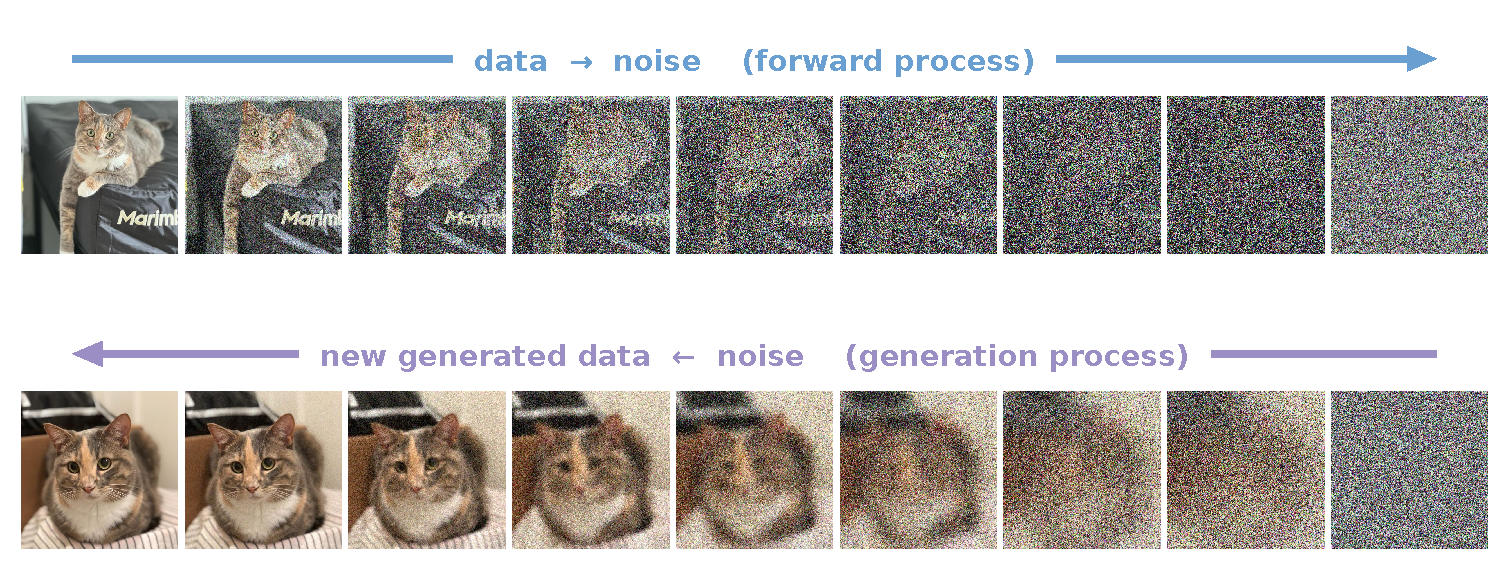
\includegraphics[width=\linewidth]{Images/PartA/diffusion_forward_vs_reverse.pdf}
    \caption{\textbfs{前向与反向扩散轨迹。}在前向过程中（上图），一个真实数据样本被噪声逐步腐蚀，经过一系列中间带噪阶段，最终变得与纯噪声难以区分。在反向过程中（下图），生成从一个全新的噪声样本开始，逐步去除噪声以产生一张新图像。反向过程并非重建训练时见过的某个特定样本，而是从全新噪声出发，逐步将其塑造成逼真的新样本。\figcredit{由作者绘制。}}
    \label{fig:ill-forward-reverse}
\end{figure}

在概述了深度生成式建模的一般目标和机制之后，我们现在转向扩散模型——一类将生成实现为从噪声到数据渐进变换的方法（见\Cref{fig:ill-forward-reverse}）。其核心思想很简单：通过不断添加噪声，可以逐步腐蚀一个数据样本，直至它与纯随机噪声无法区分。这一\emph{前向过程}将不同的数据样本映射到同一个简单的噪声空间，该空间易于采样，并作为生成的起点。在此过程中，它还创建了连接数据与噪声的一系列平滑的中间带噪阶段。在生成时，我们从这个空间中抽取一个全新的噪声样本，并通过\emph{反向（生成）过程}逐步去除噪声，最终产生一个新的数据样本。这一反向过程并不恢复某个特定的原始样本，而是从全新噪声出发，逐步将其转化为逼真的数据。我们考察三个相互关联的框架，每一个都建立在同一原理之上：一个逐步添加噪声的前向过程，以及一个由一系列逐步去噪的模型所近似的反向过程：
\begin{itemize}
    \item \textbfs{变分视角}（\Cref{ch:variational}）：源于变分自编码器（VAE）~\citep{kingma2013auto}，它通过变分目标将扩散建模为学习一个去噪过程，由此产生了去噪扩散概率模型（DDPM）~\citep{sohl2015deep,ho2020denoising}。
    \item \textbfs{分数视角}（\Cref{ch:score-based}）：植根于基于能量的模型（EBM）\\~\citep{ackley1985learning}，并发展为噪声条件分数网络（NCSN）~\citep{song2019generative}。它学习分数函数，即数据对数密度的梯度，用以指导如何逐步从样本中去除噪声。在连续时间下，\Cref{ch:score-sde} 引入了\emph{Score SDE 框架}，将这一去噪过程描述为一个随机微分方程（SDE），并将其确定性对应物描述为一个常微分方程（ODE）。这一视角将扩散建模与经典的微分方程理论联系起来，为分析和算法设计提供了清晰的数学基础。
    \item \textbfs{流视角}（\Cref{ch:flow-based}）：建立在归一化流~\citep{rezende2015variational} 之上，并由流匹配~\citep{lipman2022flow} 推广。该视角将生成建模为一个连续变换，把样本从一个简单先验传输到数据分布。这一演化由速度场通过 ODE 来支配，明确地定义了概率质量如何随时间移动。这种基于流的公式自然地超越了"先验到数据"的生成，扩展到更一般的\emph{分布到分布的转换}问题，即学习连接任意一对源分布与目标分布的流。
\end{itemize}

\begin{figure}[th!]
  \centering
  \resizebox{0.95\linewidth}{!}{%
    \begin{tikzpicture}[x=2.6cm,y=1cm,line cap=butt]
      \tikzset{>={Stealth[length=12pt,width=16pt]}}
      \def\DotR{4pt}
      \def\LabelAngle{45}
      \def\DateAboveA{32pt}
      \def\DateAboveB{32pt}
      \def\DateXShiftA{0pt}
      \def\DateXShiftB{0pt}
      \def\TextBelow{20pt}
      \def\dx{0.9}      % spacing step
      \def\XStart{0.4}  % << move EBM right by this many "x" units
      \newcommand{\nl}{\\}

      % colors
      \definecolor{PersB}{HTML}{FF7F0E} % EBM, NCSN, Score SDE
      \definecolor{PersA}{HTML}{1F77B4} % VAE, DPM, DDPM
      \definecolor{PersC}{HTML}{2CA02C} % NF, NODE, FM

      % Chronological list (even spacing by index)
      \def\Events{
        {1985/01}/{\color{PersB}{EBM}},
        {2013/12}/{\color{PersA}{VAE}},
        {2014/12}/{\color{PersC}{NF}},
        {2015/05}/{\color{PersA}{DPM}},
        {2018/06}/{\color{PersC}{NODE}},
        {2019/07}/{\color{PersB}{NCSN}},
        {2020/06}/{\color{PersA}{DDPM}},
        {2020/11}/{\color{PersB}{Score SDE}},
        {2022/10}/{\color{PersC}{FM}}
      }

      % axis
      \pgfmathsetmacro{\N}{9}
      \draw[ultra thick,-Stealth] (0,0) -- ({\XStart + (\N-1)*\dx + 0.8},0);

      % draw items
      \foreach [count=\i] \date/\desc in \Events {
        \pgfmathsetmacro{\xx}{\XStart + (\i-1)*\dx}
        \fill[black] (\xx,0) circle[radius=\DotR];

        % date above (vertical, staggered)
        \ifodd\i
          \node[above=\DateAboveA,align=center,rotate=90,inner sep=1pt,
                xshift=\DateXShiftA] at (\xx,0) {\date};
        \else
          \node[above=\DateAboveB,align=center,rotate=90,inner sep=1pt,
                xshift=\DateXShiftB] at (\xx,0) {\date};
        \fi

        % label below (45°)
        \node[below=\TextBelow,anchor=north,rotate=\LabelAngle,inner sep=1pt] at (\xx,0)
          {\shortstack[c]{\strut \desc}};
      }
    \end{tikzpicture}%
  }
  \caption{\textbfs{扩散模型各视角的时间线。}每组共享同一颜色。
  \\
\sqbullet\ 在\Cref{ch:variational} 中，{变分自编码器（VAE）}~\citep{kingma2013auto} $\to$ {扩散概率模型（DPM）}~\citep{sohl2015deep} $\to$
{DDPM}~\citep{ho2020denoising}。
 \\
\sqbullet\ 在\Cref{ch:score-based,ch:score-sde} 中，{基于能量的模型（EBM）}~\citep{ackley1985learning} $\to$ {噪声条件分数网络（NCSN）}~\citep{song2019generative} $\to$ {Score SDE}~\citep{song2020score}。  \\
\sqbullet\
在\Cref{ch:flow-based} 中，{归一化流（NF）}~\citep{rezende2015variational} $\to$ {神经 ODE（NODE）}~\citep{chen2018neural} $\to$ {流匹配（FM）}~\citep{lipman2022flow}。
\figcredit{由作者绘制。}}
  \label{fig:timeline-diffusion-perspectives-equal}
\end{figure}

尽管这些视角乍看之下各不相同，但\Cref{ch:all-equivalent} 表明它们之间存在着深刻的联系。
每一种都采用了\emph{条件化策略}，将学习目标转化为一个可处理的回归问题。
在更深层次上，它们都描述了概率分布从先验到数据的同一种时间演化。
这一演化由\emph{Fokker–Planck 方程}所支配，该方程可被视为密度的连续时间变量替换，确保了随机性与确定性公式之间的一致性。

既然扩散模型可以被视为将一个分布传输到另一个分布的方法，\Cref{ch:ot-eot} 发展了它们与经典最优传输和薛定谔桥之间的联系，后者可解释为带熵正则化的最优传输。我们回顾了静态和动态两种公式，并解释了它们与连续性方程以及 Fokker--Planck 视角的关系。对于关注实用层面的读者而言，本章是可选的；但对于希望深入研究这些联系的读者，本章提供了严格的数学背景，并指出了相关经典文献的入口。

% \ys{Some quick thoughts as I read through this part: I like how you categorize the main perspectives on diffusion into three groups, but it feels a bit odd to propose unifying them under the score SDE framework. I tend to view the score SDE framework as part of the score-based perspective. Moreover, the flow-based view emerged after the development of the score SDE framework, so it feels like an overstatement to suggest that it can be directly implied by the score SDE framework.}

%%%%%%%%%
\begin{figure}[ht!]
\begin{center}
\resizebox{\textwidth}{!}{%
\begin{tikzpicture}[
  box/.style = {draw, rounded corners, minimum width=3.6cm, minimum height=1.5cm, align=center},
  model/.style = {draw, fill=gray!20, minimum width=3.5cm, minimum height=1cm, align=center},
  arrow/.style = {ultra thick, -{Stealth[length=4mm, width=4mm]}}
  ]


   
% 2nd layer: Origin
\node[box] (vae) {Variational \\Autoencoder};
\node[box, right=1.2cm of vae] (ebm) {Energy-Based Model};
\node[box, right=1.2cm of ebm] (flow) {Normalizing Flows};

% Box around diffusion models
\node[draw, rounded corners, minimum width=13.6cm, minimum height=1.0cm, thick, above=3.5cm of ebm, label=above:{\parbox{5cm}{ \centering {Chapter}~\ref{ch:overview-dgm} 
 }}] (dgm) {Overview of Deep Generative Modeling};
  
% Top layer: Origin
\node[model, above=1.5cm of vae] (variational-based) {\large\textbfs{Variational View}};
\node[model, above=1.5cm of ebm] (score-based) {\large\textbfs{Score-Based View}};
\node[model, above=1.5cm of flow] (flow-based) {\large\textbfs{Flow-Based View}};

% Bottom layer: Diffusion Models
\node[box, below=2.2cm of vae] (ddpm) {Denoising Diffusion\\Probabilistic Model\\ (DDPM)};
\node[box, below=2.2cm of ebm] (score) {Noise Conditional\\Score Network \\(NCSN)};
\node[box, below=2.2cm of flow] (gfm) {Gaussian\\Flow Matching};

% Draw arrows
\draw[arrow] (vae.south) -- node[midway, anchor=center, yshift=3.5pt, xshift=-8pt] {\rotatebox{90}{\small {Chapter~\ref{ch:variational}}}} (ddpm.north);

\draw[arrow] (ebm.south) -- node[midway, anchor=center, yshift=3.5pt, xshift=-8pt] {\rotatebox{90}{\small {Chapter}~\ref{ch:score-based}}} (score.north);

\draw[arrow] (flow.south) -- node[midway, anchor=center, yshift=3.5pt, xshift=-8pt] {\rotatebox{90}{\small {Chapter}~\ref{ch:flow-based}}} (gfm.north);

\node[box, below=2cm of score] (scoresde) { Continuous-Time Formulation \\ (e.g., Score SDE) \\ \small {Chapter}~\ref{ch:score-sde}};

% Box around diffusion models
\node[draw, rounded corners, thick, fit={(ddpm) (score) (gfm) (scoresde)}, inner sep=0.3cm, label=below:{\parbox{5cm}{\centering\textbfs{\\ \large Unifying Principles}  \\ \vspace{0.2cm}\small {Chapter}~\ref{ch:all-equivalent} 
\begin{itemize}
    \item Conditional Strategy 
    \item Fokker-Planck Equation
\end{itemize} }}] (box) {};


\draw[ultra thick, -{Stealth[length=4mm, width=4mm]}, rounded corners=4pt] (ddpm.south) -- ++(0,-0.4) -- ([xshift=-1.0cm]scoresde.north);
\draw[ultra thick, -{Stealth[length=4mm, width=4mm]}, rounded corners=4pt] (score.south) -- ++(0,-0.4) -- (scoresde.north);
\draw[ultra thick, -{Stealth[length=4mm, width=4mm]}, rounded corners=4pt] (gfm.south) -- ++(0,-0.4) -- ([xshift=1.0cm]scoresde.north);

% Add labels
\node[align=center, left=0.5cm of box, yshift=8.3cm] {\rotatebox{90}{\textbfs{\large{Perspective}}}};
\node[align=center, left=0.5cm of box, yshift=5.5cm] {\rotatebox{90}{\textbfs{\large{Origin}}}};
\node[align=center, left=0.5cm of box] {\rotatebox{90}{\textbfs{\large{Diffusion Model}}}};
\end{tikzpicture}
 % end resizebox
    }
\end{center}
\caption{\textbfs{B 部分：扩散模型的统一与原理性视角。}此图直观地将经典生成式建模方法——变分自编码器、基于能量的模型和归一化流——与它们对应的扩散模型公式联系起来。每条纵向路径展示了一条概念脉络，最终汇聚到连续时间框架。三种视角（变分、分数和流）提供了截然不同却在数学上等价的解释。\figcredit{由作者绘制。}}
\label{fig:part-b-roadmap}
\end{figure}

%%%%%%%%%%%%%%%

%%%%%%%%%%%%%%

\paragraph{C 部分与 D 部分：控制与加速扩散采样。}

在统一了基础原理之后，我们转向利用扩散模型进行高效生成的实用层面。从扩散模型中采样对应于求解一个微分方程。然而，这一过程通常计算开销较大。C 部分和 D 部分聚焦于通过增强采样和学习型加速技术来改善生成质量、可控性和效率。



\subparagraph{C 部分：从扩散模型采样。}扩散模型的生成过程展现出独特的由粗到细的精炼：噪声被逐步去除，产生结构连贯性和细节不断增强的样本。这一特性带来了权衡。一方面，它提供了细粒度的控制；通过在学习到的、随时间变化的速度场上添加一个引导项，我们可以引导 ODE 流以反映用户意图，使采样变得可控。另一方面，所需的迭代积分使得采样相比单步生成器要缓慢。
本部分聚焦于在推理时改进生成过程，且无需重新训练。
\begin{itemize}
    \item \textbfs{引导生成}（\Cref{ch:guidance}）\textbfs{:} 诸如分类器引导和无分类器引导等技术，使得生成过程能够以用户定义的目标或属性为条件。在此基础上，我们接下来讨论如何使用偏好数据集进一步将扩散模型与这些偏好相对齐。
    \item \textbfs{用数值求解器实现快速生成}（\Cref{ch:solvers}）\textbfs{:} 使用先进的数值求解器可以在更少的步数内近似反向过程，从而显著加速采样，在降低开销的同时保持质量。
\end{itemize}
\subparagraph{D 部分：学习快速的生成式模型。}除了改进现有的采样算法，我们还研究如何直接学习能够近似扩散过程的快速生成器。
\begin{itemize}
    \item \textbfs{基于蒸馏的方法}（\Cref{ch:distillation}）：该方法聚焦于训练一个学生模型来模仿一个预训练的、缓慢的扩散模型（教师模型）的行为。其目标不是缩小教师模型的规模，而是以远少得多的积分步数（通常只有几步甚至一步）重现其采样轨迹或输出分布。
    \item \textbfs{从零开始学习}（\Cref{ch:fast-scratch}）\textbfs{:} 既然扩散模型中的采样可以被视为求解一个 ODE，该方法便从零开始直接学习该解的映射（即流映射），而无需依赖教师模型。学习到的映射可以直接将噪声变为数据，或更一般地在求解轨迹上执行任意时刻到任意时刻的跳跃。
\end{itemize}


% \ys{Should we call it ``distillation-based methods''? Not sure distillation is one type of post-training. That said, we may indeed want to discuss post-training techniques for diffusion models in nearby sections on ``steering generation''. }

\paragraph{尾声：超越连续状态空间上的扩散。}
我们在\Cref{ch:epilogue} 中明确指出贯穿全书的核心原理。从本质上讲，扩散建模并不绑定于某一种特定的噪声类型、模型类别，甚至不绑定于连续状态空间。它所研究的，是概率质量在一个预先规定的时间相关的前向腐蚀过程下如何演化，以及这种演化如何被反转、被近似、或被用于生成。在连续设定下，这一原理通过变量替换公式、连续性方程和 Fokker--Planck 方程体现。在离散设定下，相同结构性作用由转移核、连续时间马尔可夫链和主方程承担。

最后这一章还表明，本书贯穿始终所发展的三种视角——即变分、分数和流视角——超越了连续数据建模。即便对于文本、蛋白质序列以及其他基于词元的对象等离散数据，人们仍然可以通过变分目标、类似分数的比率或反向速率刻画，以及类似流的传输视角来 formulate 反向建模。数学对象改变了，但底层原理并未改变。如此一来，尾声既是全书在概念上的总结，也指向了生成式建模更广阔图景的展望。


\paragraph{附录。}
为确保这段旅程对所有读者都易于理解，附录提供了基础概念的背景知识。\Cref{app:de} 提供了一份关于微分方程的速成课程，微分方程已成为扩散模型的语言。

尽管扩散模型视角和起源各异，其背后的核心洞见在于\emph{变量替换公式}。这一基础自然延伸到更深层的概念，如\emph{Fokker--Planck 方程}和\emph{连续性方程}，它们描述了概率密度如何由函数（离散时间）或微分方程（连续时间）定义的映射所变换和演化。
\Cref{app:continuity} 提供了一份平易近人的介绍，将这些基础思想桥接到更高级的概念。
在\Cref{app:Ito} 中，我们呈现了扩散模型背后两个强大却常被忽视的工具：\emph{Itô 公式}和\emph{Girsanov 定理}，它们为 Fokker--Planck 方程和反向采样过程提供了严格的支持。
最后，\Cref{app:proof} 汇集了正文章节中部分命题和定理的证明。


% \paragraph{What this Book Covers and What Does Not?}

% Overall, from the top-down viewpoint this book covers from the core principle of ``constructing the dynamics that transporting in continuous time from the simple prior distribution to the data distribution while making the distribution at each time snapshot matches with the distributions of pre-scribed process from data-to-noise''. Starting from this diffusion-modeling principle, we discuss the stochastic/deterministic flow to realize the sampling transportation, and establish the controllable and faster way of achieving this transportation.  We do not cover the detailed practical implementations, engineering know-hows, models or architectureal selections, datasets benchmarking, or domain-specific applications. 



\paragraph{本书涵盖的内容与不涵盖的内容。}
我们追求经久耐用。从自顶向下的视角来看，本书从一个单一原理出发：构造连续时间的动力学，将一个简单先验传输到数据分布，同时确保每一时刻的边缘分布与一个预先规定的前向过程（从数据到噪声）所诱导的边缘分布相匹配。从这一原理出发，我们发展了实现采样的随机流和确定性流，展示了如何引导轨迹（引导），并解释了如何加速它（数值求解器）。然后，我们研究受扩散启发的快速生成器，包括蒸馏方法和流映射模型。借助这些工具，读者可以将新论文纳入一个共同模板，理解方法为何有效，并设计出改进的模型。

我们并不试图对扩散模型文献进行穷尽式的综述，也不罗列架构、训练实践、超参数，不对各方法的经验结果进行比较，不涵盖数据集和排行榜，不描述特定领域或模态的应用，不讨论系统级部署，不提供大规模训练的配方，也不讨论硬件工程。这些主题演变迅速，更适合由专题综述、开放仓库和实现指南来涵盖。







% \begin{figure}[th!]
% \caption{\textbfs{Part C. Sampling with Diffusion Models.} \Cref{ch:score-sde} shows that diffusion model sampling is equivalent to solving an ODE. From this view, the \textit{left branch} interprets guided generation as steering the velocity field with auxiliary signals. As this process involves solving differential equations, it is inherently slow. To mitigate this, the \textit{middle branch} employs classical numerical solvers to accelerate sampling by efficiently estimating the integral using a pre-trained model $\rvv$. \\
% \textbfs{Part D. Learning a Fast Diffusion-Based Generator.} The \textit{right branch} takes a different route: directly learning to approximate the ODE solution or its distribution at $t=0$, either using a pre-trained model or training from scratch. The latter yields a standalone generator that avoids costly sampling.
% }
% \begin{center}
% \resizebox{\textwidth}{!}{% 
% \centering
% \begin{tikzpicture}[
%     box/.style={rectangle, draw, thick, minimum width=3cm, minimum height=2cm, align=center},
%     topbox/.style={rectangle, draw, thick, minimum width=12cm, minimum height=1.5cm, align=center},
%     arrow/.style={->, thick},
%     roundbox/.style={rectangle, draw, thick, rounded corners=10pt, minimum width=4cm, minimum height=3cm, align=center}
% ]

% % Top box
% \node[topbox, label=above:{\parbox{5cm}{\centering  {Chapter}~\ref{ch:score-sde}}}] (top) at (0,4) {\\
% \textbfs{Generation with Diffusion Model $\mathbf{v}(\rvx, t)$} \\[0.3cm]
% $\Longleftrightarrow$ Solve ODE backward from $t = T$ to $0$ with $\mathbf{x}(T) \sim p_{\mathrm{prior}}$: \\[0.2cm]
% $\displaystyle\frac{\diff\mathbf{x}(t)}{\diff t} = \mathbf{v}(\mathbf{x}(t), t)$ \\[0.3cm]
% $\displaystyle\Longleftrightarrow \mathbf{x}(0) = \mathbf{x}(T) + \int_0^T \mathbf{v}(\mathbf{x}(t), t)\diff t$
% };

% % Three bottom boxes
% \node[roundbox, label=below:{\parbox{5cm}{\centering  {Chapter}~\ref{ch:guidance} 
%  }}] (left) at (-6,-2) {
% \\ \large\textbfs{Steering Generation} \\[0.4cm]
% \parbox{5cm}{
% \begin{align*}
%     \displaystyle\mathbf{x}(0) &= \mathbf{x}(T) + \int_0^T [\mathbf{v}(\mathbf{x}(t), t) \\ 
%     &\qquad \textcolor{darkgray}{+ \textbf{Guidance}}] \diff t
% \end{align*}}
% };

% \node[roundbox, label=below:{\parbox{5cm}{\centering {Chapter}~\ref{ch:solvers} 
%  }}] (center) at (0,-2) {
% \\ \large\textbfs{Fast Generation} \\
% \large\textbfs{with Numerical Solvers} \\[-0.6cm]
% $\displaystyle\mathbf{x}(0) = \mathbf{x}(T) + \eqnmarkbox[Plum]{velocity}{\int_0^T \mathbf{v}(\mathbf{x}(t), t)\diff t}$ \\[-0.8cm]
% Estimating the integral
% };

% \node[roundbox, label=below:{\parbox{5cm}{\centering  {Chapter}~\ref{ch:distillation} and {Chapter}~\ref{ch:fast-scratch} 
%  }}] (right) at (6,-2) {
% \\ \large\textbfs{Learning a Fast} \\
% \large\textbfs{Diffusion-Based Generator} \\[-0.6cm]
% $\displaystyle\mathbf{x}(0) = \eqnmarkbox[Pink]{target}{\mathbf{x}(T) + \int_0^T \mathbf{v}(\mathbf{x}(t), t)\diff t}$ \\[-0.8cm]
% Learning the Integral
% };

% % Arrows
% \draw[ultra thick, -{Stealth[length=4mm, width=4mm]}, rounded corners=4pt] (top.south) -- ++(-6,-1) -- (left.north);
% \draw[ultra thick, -{Stealth[length=4mm, width=4mm]}, rounded corners=4pt] (top.south) -- (center.north);
% \draw[ultra thick, -{Stealth[length=4mm, width=4mm]}, rounded corners=4pt] (top.south) -- ++(6,-1) -- (right.north);

% \end{tikzpicture}
% }
% \end{center}
% \label{fig:part-c-d-roadmap}
% \end{figure}

% \se{i don't think this figure will make sense to readers that don't already know diffusion}

% \se{btw, i think it's integral not integration}
%%%%%%%%%%%%%%%



